

\tikzset{every picture/.style={line width=0.75pt}} %set default line width to 0.75pt        

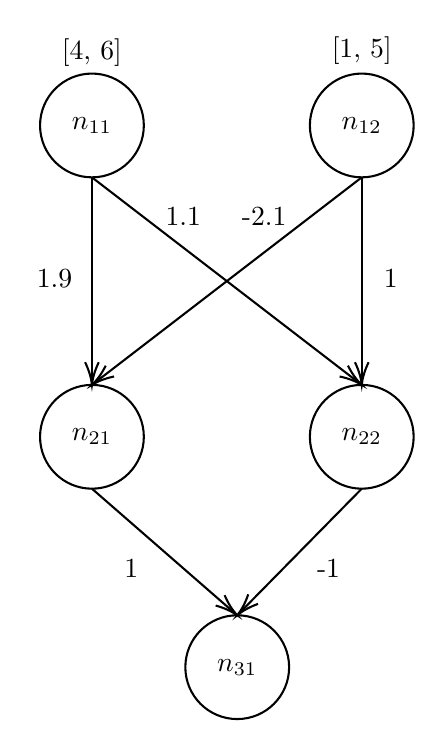
\begin{tikzpicture}[x=0.75pt,y=0.75pt,yscale=-1,xscale=1]
%uncomment if require: \path (0,461); %set diagram left start at 0, and has height of 461

%Shape: Circle [id:dp3477853434711644] 
\draw   (40,55.33) .. controls (40,41.53) and (51.19,30.33) .. (65,30.33) .. controls (78.81,30.33) and (90,41.53) .. (90,55.33) .. controls (90,69.14) and (78.81,80.33) .. (65,80.33) .. controls (51.19,80.33) and (40,69.14) .. (40,55.33) -- cycle ;
%Shape: Circle [id:dp340302200627272] 
\draw   (170,55.33) .. controls (170,41.53) and (181.19,30.33) .. (195,30.33) .. controls (208.81,30.33) and (220,41.53) .. (220,55.33) .. controls (220,69.14) and (208.81,80.33) .. (195,80.33) .. controls (181.19,80.33) and (170,69.14) .. (170,55.33) -- cycle ;
%Shape: Circle [id:dp8648816362042863] 
\draw   (170,205.33) .. controls (170,191.53) and (181.19,180.33) .. (195,180.33) .. controls (208.81,180.33) and (220,191.53) .. (220,205.33) .. controls (220,219.14) and (208.81,230.33) .. (195,230.33) .. controls (181.19,230.33) and (170,219.14) .. (170,205.33) -- cycle ;
%Shape: Circle [id:dp0718016291504322] 
\draw   (40,205.33) .. controls (40,191.53) and (51.19,180.33) .. (65,180.33) .. controls (78.81,180.33) and (90,191.53) .. (90,205.33) .. controls (90,219.14) and (78.81,230.33) .. (65,230.33) .. controls (51.19,230.33) and (40,219.14) .. (40,205.33) -- cycle ;
%Shape: Circle [id:dp36074725334199054] 
\draw   (110,316.33) .. controls (110,302.53) and (121.19,291.33) .. (135,291.33) .. controls (148.81,291.33) and (160,302.53) .. (160,316.33) .. controls (160,330.14) and (148.81,341.33) .. (135,341.33) .. controls (121.19,341.33) and (110,330.14) .. (110,316.33) -- cycle ;
%Straight Lines [id:da4830467038626779] 
\draw    (65,80.33) -- (65,178.33) ;
\draw [shift={(65,180.33)}, rotate = 270] [color={rgb, 255:red, 0; green, 0; blue, 0 }  ][line width=0.75]    (10.93,-3.29) .. controls (6.95,-1.4) and (3.31,-0.3) .. (0,0) .. controls (3.31,0.3) and (6.95,1.4) .. (10.93,3.29)   ;

%Straight Lines [id:da6559633273133572] 
\draw    (195,80.33) -- (195,178.33) ;
\draw [shift={(195,180.33)}, rotate = 270] [color={rgb, 255:red, 0; green, 0; blue, 0 }  ][line width=0.75]    (10.93,-3.29) .. controls (6.95,-1.4) and (3.31,-0.3) .. (0,0) .. controls (3.31,0.3) and (6.95,1.4) .. (10.93,3.29)   ;

%Straight Lines [id:da6702947498516574] 
\draw    (195,80.33) -- (66.59,179.11) ;
\draw [shift={(65,180.33)}, rotate = 322.43] [color={rgb, 255:red, 0; green, 0; blue, 0 }  ][line width=0.75]    (10.93,-3.29) .. controls (6.95,-1.4) and (3.31,-0.3) .. (0,0) .. controls (3.31,0.3) and (6.95,1.4) .. (10.93,3.29)   ;

%Straight Lines [id:da410799694588483] 
\draw    (65,80.33) -- (193.41,179.11) ;
\draw [shift={(195,180.33)}, rotate = 217.57] [color={rgb, 255:red, 0; green, 0; blue, 0 }  ][line width=0.75]    (10.93,-3.29) .. controls (6.95,-1.4) and (3.31,-0.3) .. (0,0) .. controls (3.31,0.3) and (6.95,1.4) .. (10.93,3.29)   ;

%Straight Lines [id:da3771185529221218] 
\draw    (195,230.33) -- (136.4,289.91) ;
\draw [shift={(135,291.33)}, rotate = 314.53] [color={rgb, 255:red, 0; green, 0; blue, 0 }  ][line width=0.75]    (10.93,-3.29) .. controls (6.95,-1.4) and (3.31,-0.3) .. (0,0) .. controls (3.31,0.3) and (6.95,1.4) .. (10.93,3.29)   ;

%Straight Lines [id:da5059391581413158] 
\draw    (65,230.33) -- (133.49,290.02) ;
\draw [shift={(135,291.33)}, rotate = 221.07] [color={rgb, 255:red, 0; green, 0; blue, 0 }  ][line width=0.75]    (10.93,-3.29) .. controls (6.95,-1.4) and (3.31,-0.3) .. (0,0) .. controls (3.31,0.3) and (6.95,1.4) .. (10.93,3.29)   ;


% Text Node
\draw (47,129) node  [align=left] {1.9};
% Text Node
\draw (109,99) node  [align=left] {1.1};
% Text Node
\draw (148,99) node  [align=left] {\mbox{-}2.1};
% Text Node
\draw (209,129) node  [align=left] {1};
% Text Node
\draw (84,269) node  [align=left] {1};
% Text Node
\draw (179,269) node  [align=left] {\mbox{-}1};
% Text Node
\draw (65,55.33) node   {$n_{11}$};
% Text Node
\draw (195,55.33) node   {$n_{12}$};
% Text Node
\draw (65,205.33) node   {$n_{21}$};
% Text Node
\draw (195,205.33) node   {$n_{22}$};
% Text Node
\draw (135,316.33) node   {$n_{31}$};
% Text Node
\draw (65,20.33) node  [align=left] {[4, 6]};
% Text Node
\draw (195,19.33) node  [align=left] {[1, 5]};


\end{tikzpicture}
